
% ***************************************************
% Example of an internal chapter
% ***************************************************
%This is an internal chapter of the thesis.
%If you have a long title, you can supply an abbreviated version to print in the Table of Contents using the optional argument to the \chapter command.
\chapter[Methodology]{Methodology}
\label{chap:methodology}	%CREATE YOUR OWN LABEL.
\pagestyle{headings}

This chapter will detail the design decisions and steps taken to complete the project. 


\section{FPGA}
The Digilent Nexys A7-100T FPGA development board was used for this project. Namely, this board featured a Xilinx Artix 7 100T FPGA (part number XC7A100T-1CSG324C), LAN8720A 100MBit/s RMII PHY and PMOD (auxiliary outputs) amoung other IO. 


\begin{figure}[h]
    \centering
    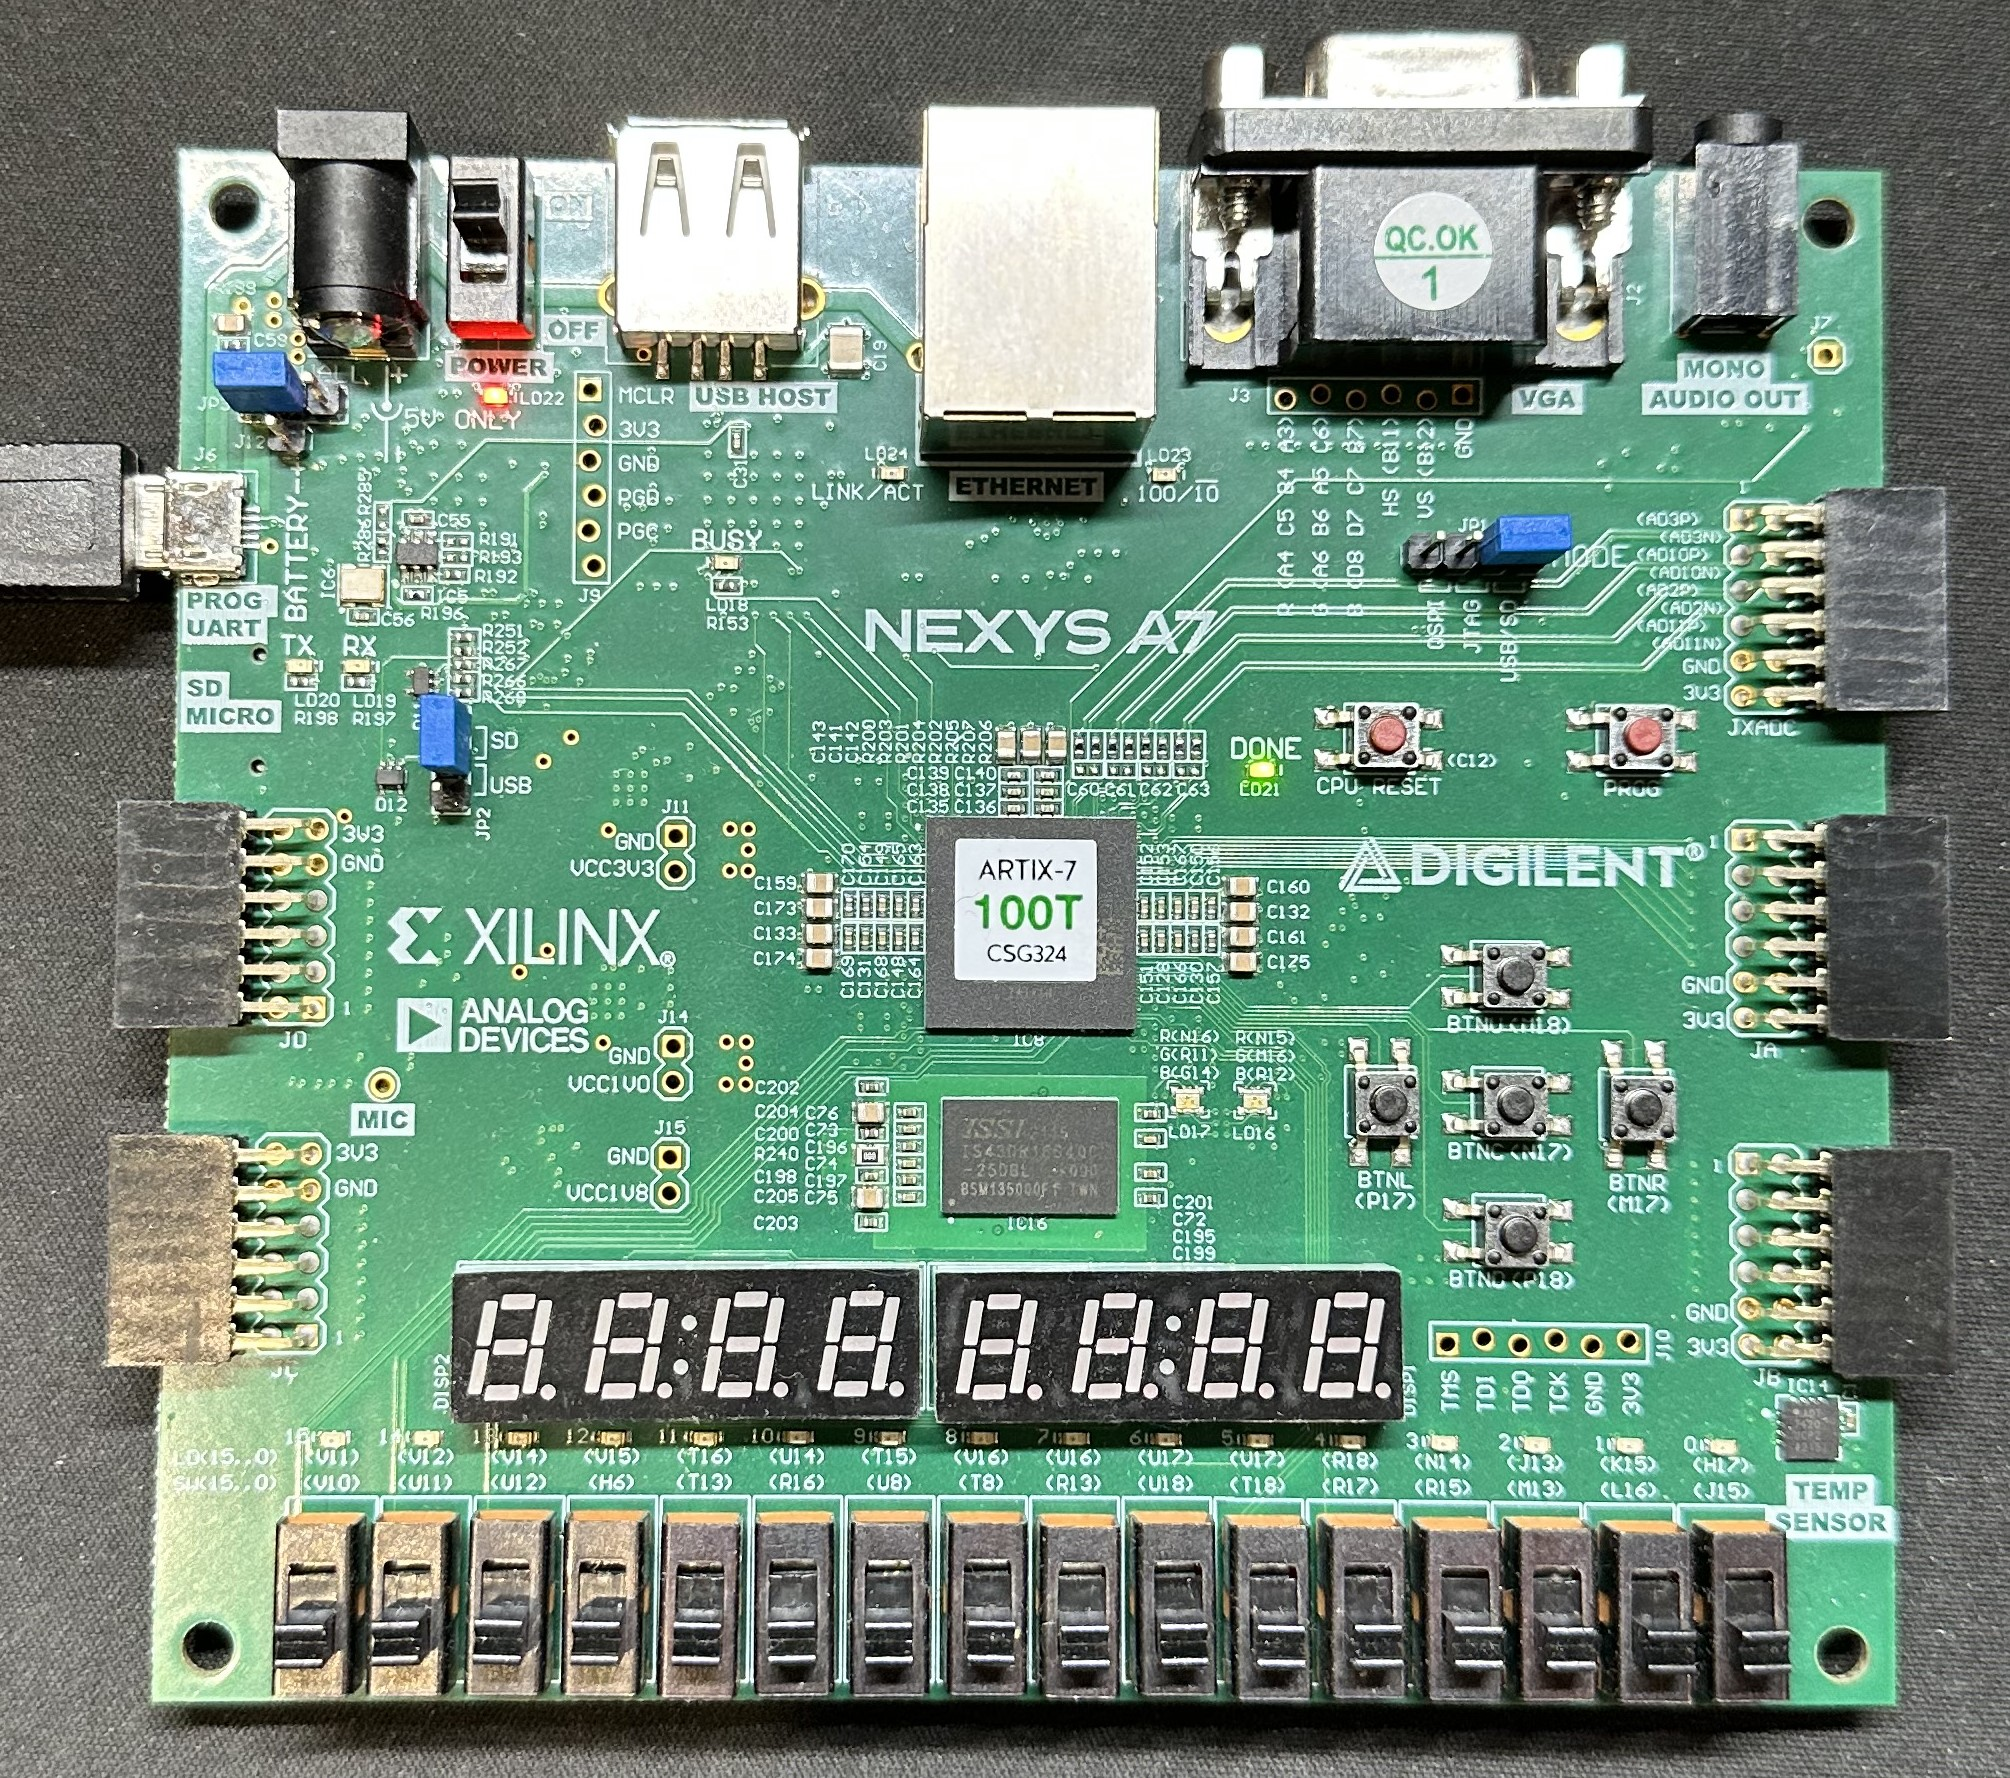
\includegraphics[width=0.65\textwidth]{Images/nexysa7_board.jpg}
    \caption[Digilent Nexys A7 FPGA development board]{Digilent Nexys A7 FPGA development board.}
    \label{fig:fpga_dev_board}
\end{figure}


As a packet filter, a second Ethernet interface was required. Hence, a secondary LAN8720A breakout board was used and connected using the PMOD connectors on the development board. 


\subsubsection{PMOD Interface}

Have some eye diagrams here to show the validity of using PMOD.

\section{System on Chip}

The NEORV32 processor by GitHub user stnolting was used in this project. It's a highly configurable microcontroller-like SoC. 


\subsection{MicroSD card}
The web assets were stored on a MicroSD card. SD cards have 2 modes of operation: native SD mode and SPI mode. To keep things simple, the microSD card was connected to with SPI mode. 




\section{Ethernet Media Access Controller}
The advantage of using an FPGA is that custom hardware can be designed for specific tasks. In this design the MAC layer was done purely in hardware to free up the microprocessor by handling all of the lower level logic. 

This MAC was implemented as a memory-mapped perhipheral which used the MCU's Wishbone B4 classic interface. This then made it easily accessable over the memory address space of the MCU.  



\section{Packet Classifier}

To further save MCU resources, the packet classification was done in hardware. Not only did this reduce the load on the MCU itself - giving it more time to do other things - it allowed the interface to run at \textit{'wirespeed'}. That is, at the full speed of the interface - 100Mbit/s. 

This was possible by having the rulset been evaluated in parallel as the data is coming into the firewall. This method however is not suitable for large rulesets as the fan-in and fan-out limit the maximum number of parallel comparisons. For every new rule, the number of gates grows exponentially. Hence a design decision of a maximum ruleset of size 8 was chosen. 

The way this classifier was designed was to be a \textit{'default-block'} where all connections were blocked except for the ones specifically whitelisted in the ruleset. 

The specific rules had a few options, namely the source IP address, destination IP address, source port, destination port and protocol could be configured. In addition to these, each field had a wildcard operator which allowed all values for that specific option to be classified. 

A block diagram of the classifier can be seen in figure XX below. To control the flow of the packets, a buffer was used on the input to store the packet as it was coming in. At the same time the classifier would start classifying the packet. If allowed, then the packet would be moved on to another buffer before been sent out the other interface. If the packet was blocked, then the data would be dropped by clearing the buffers and then just ignoring the remainder of the incomming packet. 





\section{Firmware}

\subsection{Real Time Operating System}
In addition to simplifying the project, and RTOS was used as this would allow the use of network TCP stacks. The RTOS that was used in this design was FreeRTOS V10.4.4 due to its familirity and compatability with the NEORV32 MCU.


\subsection{Network Stack}
There were two main options for the network stack, LwIP and FreeRTOS-Plus-TCP. The main concern with LwIP was that it was not threadsafe and had memory issues. In addition to this, as FreeRTOS was chosen as the RTOS, their own TCP stack was used as it was thought to have tighter integration. 


\subsection{Webserver}
A simple HTTP webserver running on top of a TCP server was used to serve the webpages for the project. 


\subsection{Improvements}

\begin{itemize}
    \item Bidirectional filtering - currently only doing incomming filtering
\end{itemize}